\section{Introdução ao LibreOffice Calc}

\begin{frame}{Introdução}
	\begin{block}{}
		O Calc é o programa de \textbf{planilhas eletrônicas} incluído no LibreOffice.
		
		\medskip
		
		Mas \textbf{para que serve} uma planilha eletrônica?
		\begin{itemize}
			\item \textbf{Organizar dados} em tabelas;
			\item \textbf{fazer cálculos}, \textbf{análisar} e \textbf{gerenciar dados};
			\item \textbf{automatizar tarefas};
			\item \textbf{filtrar informações};
			\item \textbf{gerar gráficos} a partir de resultados.
		\end{itemize}
	\end{block}
	
	\centering
	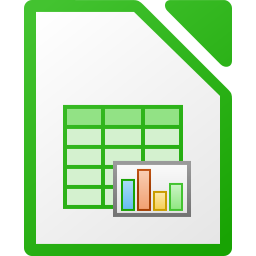
\includegraphics[width=0.25\linewidth]{Figuras/Ch06/fig1}
\end{frame}


\begin{frame}{Área de trabalho do Calc}
	\centering
	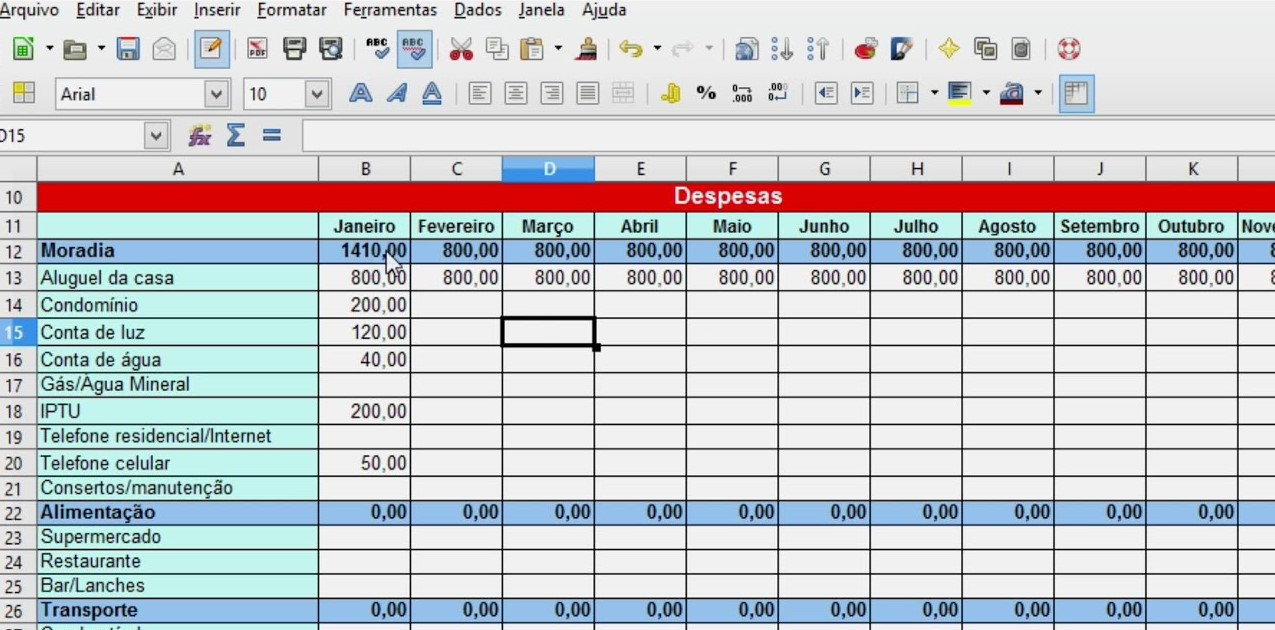
\includegraphics[width=1\linewidth]{Figuras/Ch06/fig0}
\end{frame}


\begin{frame}{Área de trabalho do Calc}
	\begin{block}{}
		Composição padrão da área ou ambiente de trabalho:
		\begin{enumerate}
			\item Planilha eletrônica.
		\end{enumerate}
	\end{block}
	
	\centering
	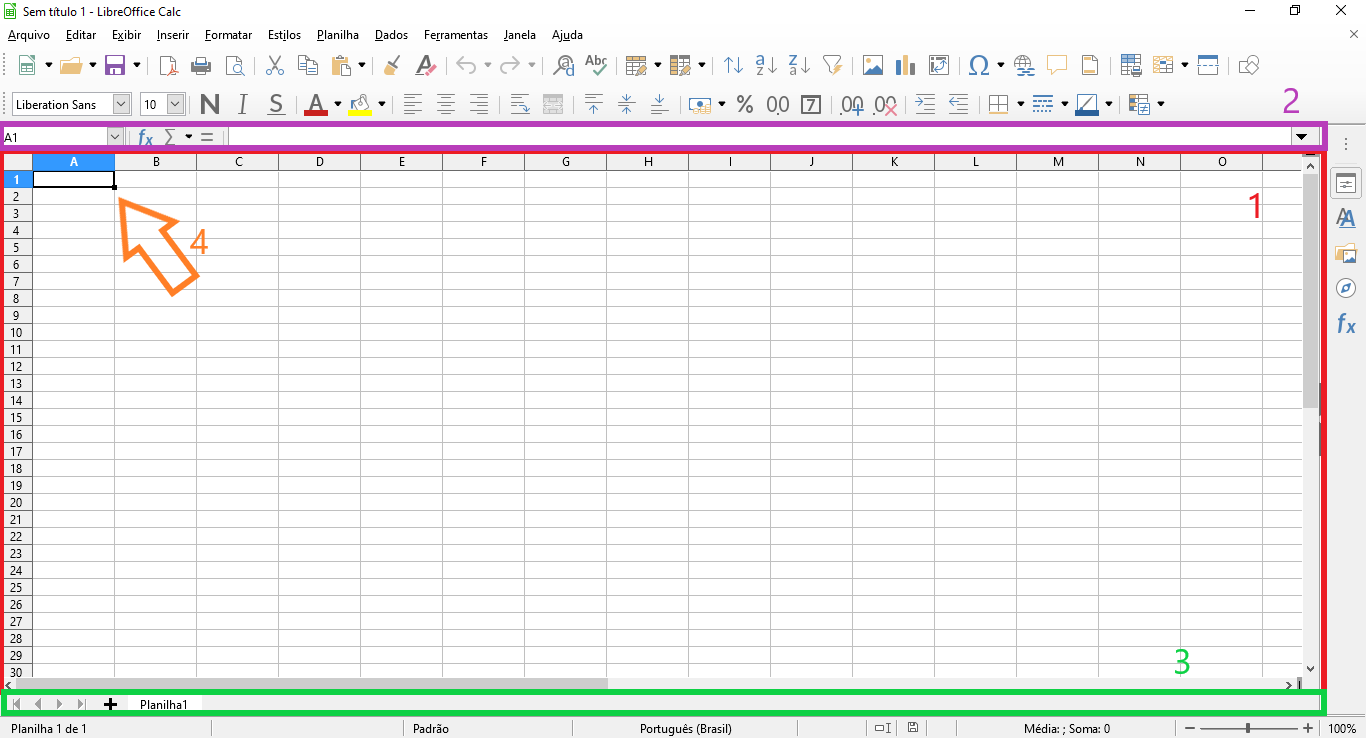
\includegraphics[width=0.9\linewidth]{Figuras/Ch06/fig2}
\end{frame}


\begin{frame}{Área de trabalho do Calc}
	\begin{block}{}
		\begin{enumerate}
			\setcounter{enumi}{1}
			\item Barra de fórmulas.
		\end{enumerate}
	\end{block}
	
	\centering
	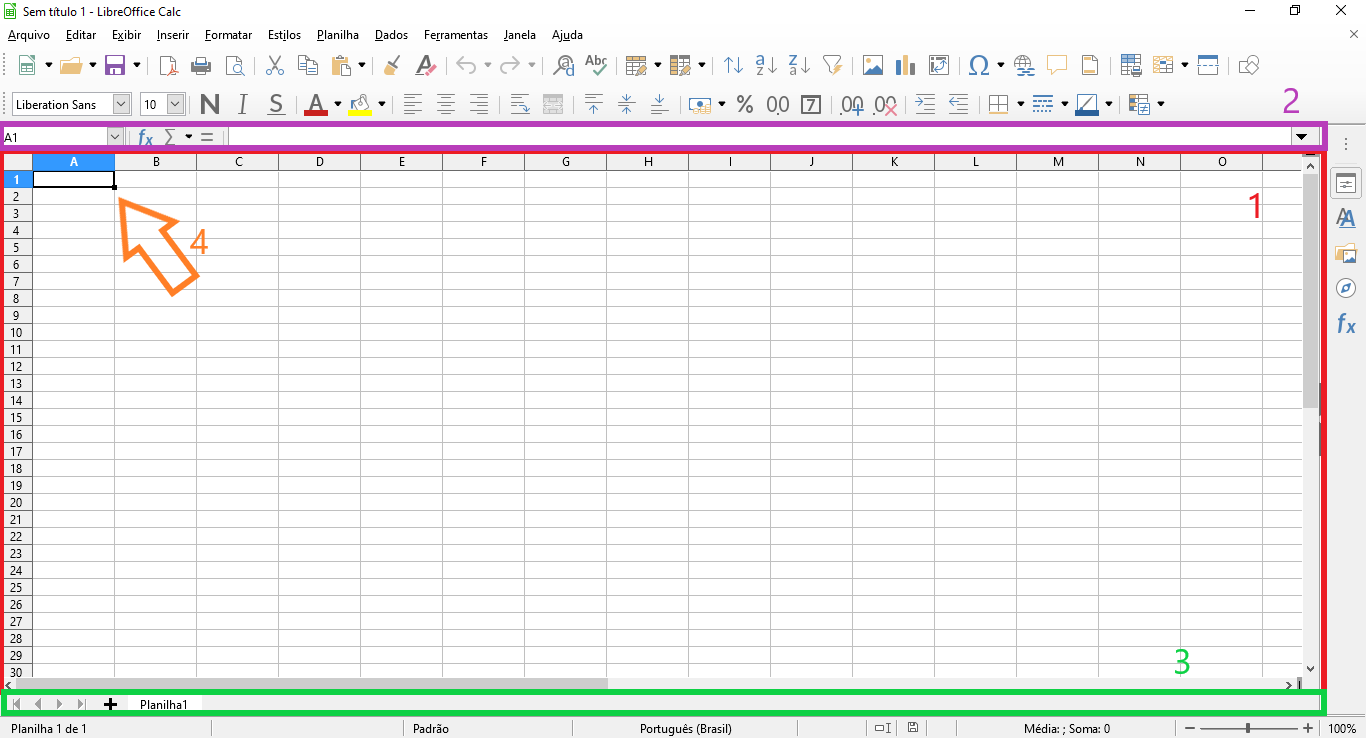
\includegraphics[width=0.95\linewidth]{Figuras/Ch06/fig2}
\end{frame}


\begin{frame}{Área de trabalho do Calc}
	\begin{block}{}
		\begin{enumerate}
			\setcounter{enumi}{2}
			\item Barra de planilhas.
		\end{enumerate}
	\end{block}
	
	\centering
	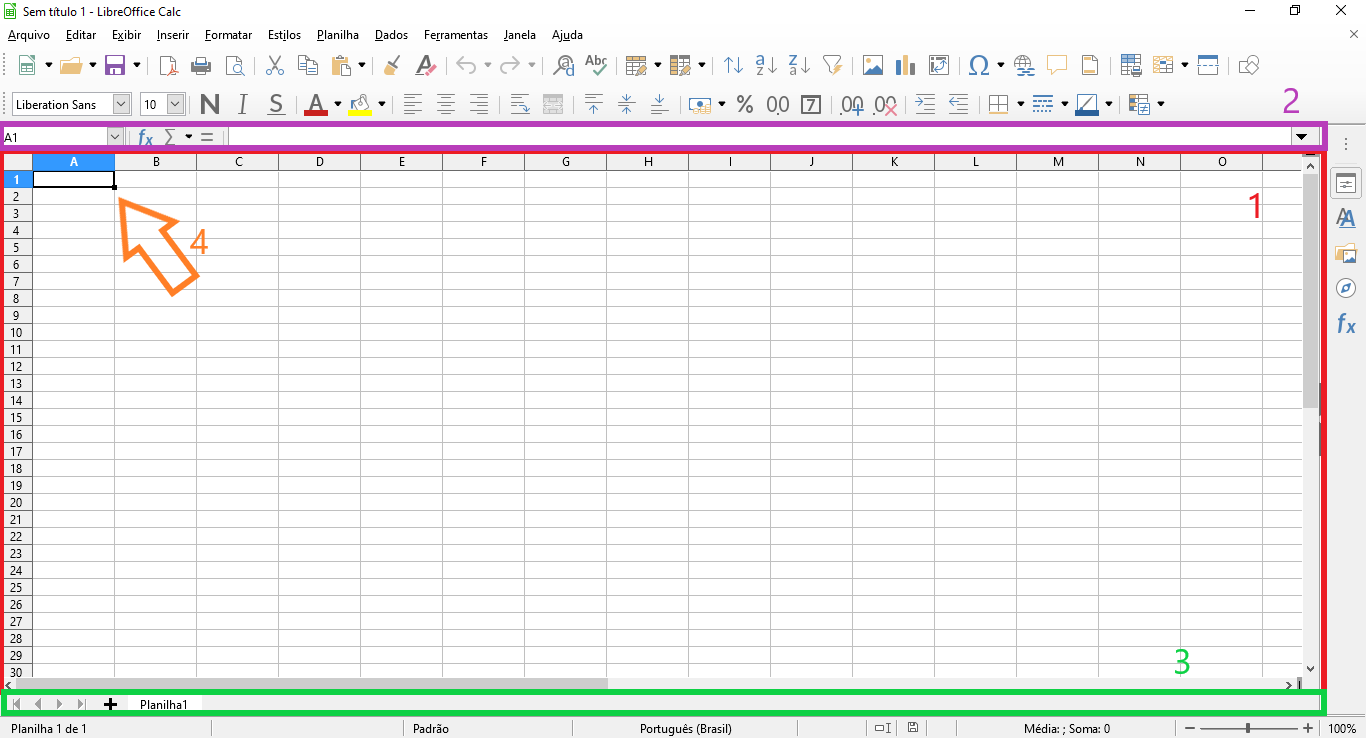
\includegraphics[width=0.95\linewidth]{Figuras/Ch06/fig2}
\end{frame}


\begin{frame}{Área de trabalho do Calc}
	\begin{block}{}
		\begin{enumerate}
			\setcounter{enumi}{3}
			\item Ponteiro da célula.
		\end{enumerate}
	\end{block}
	
	\centering
	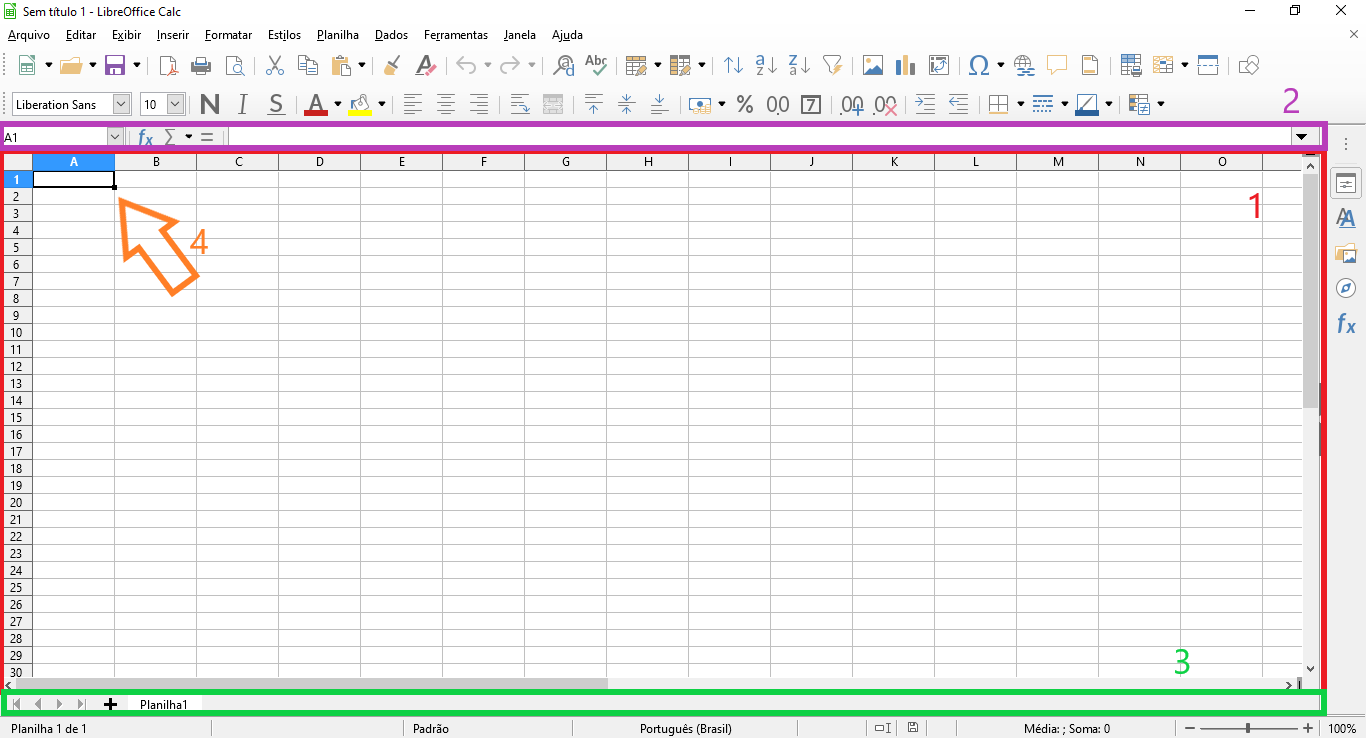
\includegraphics[width=0.95\linewidth]{Figuras/Ch06/fig2}
\end{frame}


\begin{frame}{Área de trabalho do Calc}
	\begin{block}{Composição da planilha eletrônica}
		\begin{itemize}
			\item \textbf{Colunas:} representadas por letras maiúsculas, no sentido vertical.
			\item \textbf{Linhas:} representadas por números em ordem crescente (1, 2, 3, 4...), no sentido horizontal.
			\item \textbf{Células:} são unidades onde entramos com os dados.
			\item \textbf{Célula ativa:} É a célula onde se encontra o cursor no instante da entrada de dados.
		\end{itemize}
	\end{block}
	
	\centering
	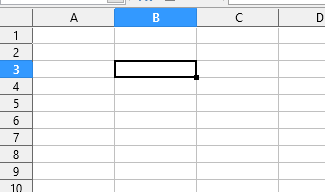
\includegraphics[width=0.5\linewidth]{Figuras/Ch06/fig3}
\end{frame}


\begin{frame}{Endereço da célula}
	\begin{block}{}
		O endereço único de cada célula é dado pela coluna e linha.
		
		\medskip
		
		Exemplos:
		\begin{itemize}
			\item D4 – coluna D e linha 4.
			\item F14 – coluna F e linha 14.
		\end{itemize}
	\end{block}
	
	\bigskip
	
	\centering
	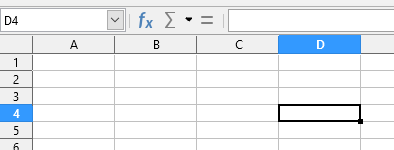
\includegraphics[width=1\linewidth]{Figuras/Ch06/fig4}
\end{frame}


\begin{frame}{Alça de preenchimento}
	\begin{block}{}
		Marca existente no canto inferior direito da célula que serve para fazer \textbf{progressão} ou \textbf{cópia} de dados.
		\begin{itemize}
			\item 1, 2, 3...
		\end{itemize}
	\end{block}
	
	\centering
	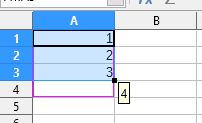
\includegraphics[width=0.7\linewidth]{Figuras/Ch06/fig5}
\end{frame}


\begin{frame}{Alça de preenchimento}
	\begin{block}{}
		\begin{itemize}
			\item Segunda-feira, terça-feira...
		\end{itemize}
	\end{block}

	\bigskip
	
	\centering
	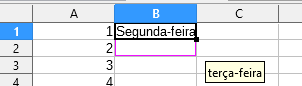
\includegraphics[width=1\linewidth]{Figuras/Ch06/fig6}
\end{frame}


\begin{frame}{Alça de preenchimento}
	\begin{block}{}
		\begin{itemize}
			\item Janeiro, Fevereiro, Março...
		\end{itemize}
	\end{block}
	
	\bigskip
	
	\centering
	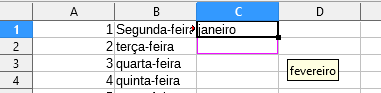
\includegraphics[width=1\linewidth]{Figuras/Ch06/fig7}
\end{frame}


\begin{frame}{Alça de preenchimento}
	\begin{block}{}
		\begin{itemize}
			\item cachorro, cachorro, cachorro...
		\end{itemize}
	\end{block}
	
	\centering
	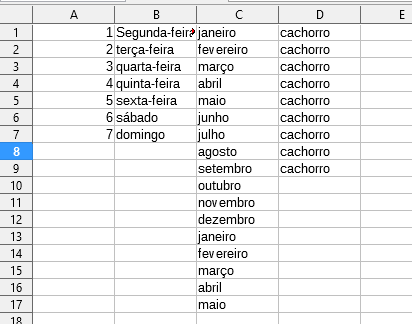
\includegraphics[width=0.7\linewidth]{Figuras/Ch06/fig8}
\end{frame}


\begin{frame}{Alça de preenchimento}
	\begin{block}{}
		\begin{itemize}
			\item Também é possível fazer várias sequências simultaneamente.
		\end{itemize}
	\end{block}
	
	\bigskip
	
	\centering
	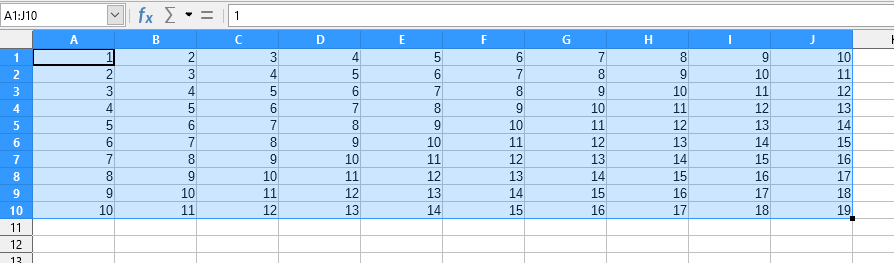
\includegraphics[width=1\linewidth]{Figuras/Ch06/fig9}
\end{frame}


\begin{frame}{Movimentação e seleção}
	\begin{block}{}
		\begin{itemize}
			\item \textbf{Home:}
			Movimenta o ponteiro de célula para a primeira coluna (A) da linha em que se encontra o cursor.
			\item \textbf{Ctrl + Home:}
			Movimenta o ponteiro de célula até a primeira célula da planilha (A1).
		\end{itemize}
	\end{block}
	
	\begin{minipage}{0.49\linewidth}
		\centering
		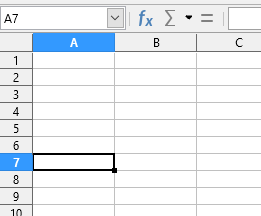
\includegraphics[width=1\linewidth]{Figuras/Ch06/fig10}
	\end{minipage}\hfill
	\begin{minipage}{0.49\linewidth}
		\centering
		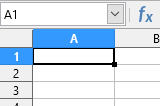
\includegraphics[width=1\linewidth]{Figuras/Ch06/fig11}
	\end{minipage}
\end{frame}


\begin{frame}{Movimentação e seleção}
	\begin{block}{}
		\begin{itemize}
			\item \textbf{Shift + Home:}
			Seleciona as células a partir de onde se encontra o ponteiro até a célula da primeira coluna da linha em que se encontra o cursor.
			\item \textbf{Ctrl + Shift + Home:}
			Seleciona todas as células entre a célula que se encontra o ponteiro até a primeira célula da planilha (A1).
		\end{itemize}
	\end{block}

	\bigskip
	
	\begin{minipage}{0.49\linewidth}
		\centering
		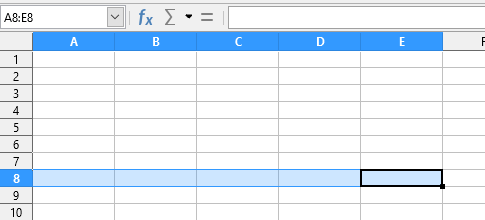
\includegraphics[width=1\linewidth]{Figuras/Ch06/fig12}
	\end{minipage}\hfill
	\begin{minipage}{0.49\linewidth}
		\centering
		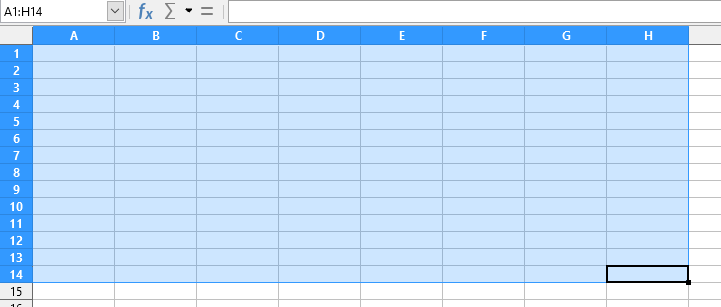
\includegraphics[width=1\linewidth]{Figuras/Ch06/fig13}
	\end{minipage}
\end{frame}


\begin{frame}{Movimentação e seleção}
	\begin{block}{}
		\begin{itemize}
			\item Mesmo raciocínio para a tecla de fluxo de texto \textbf{End}.
			\item \textbf{PgDn:} Movimenta o ponteiro de célula para baixo, de 30 em 30 células.
			\item \textbf{PgUp:} Movimenta o ponteiro de célula para cima, de 30 em 30 células.
		\end{itemize}
	\end{block}
	
	\centering
	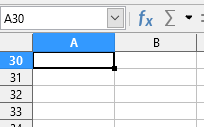
\includegraphics[width=0.7\linewidth]{Figuras/Ch06/fig14}
\end{frame}


\begin{frame}{Movimentação e seleção}
	\begin{block}{}
		\begin{itemize}
			\item \textbf{$ \bm{\to} $:} Movimenta o ponteiro de célula para a direita.
			\item \textbf{Shift + $\bm{\to}$:} Movimenta o ponteiro de célula para a direita, selecionando todas as células por onde passa.
			\item \textbf{Ctrl + $\bm{\to}$:} Movimenta o ponteiro de célula para a última coluna da linha em que se encontra o cursor.
		\end{itemize}
	\end{block}
	
	\centering
	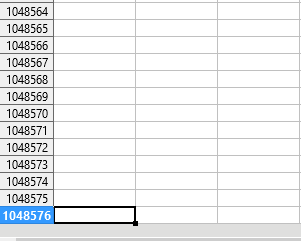
\includegraphics[width=0.5\linewidth]{Figuras/Ch06/fig15}
\end{frame}


\begin{frame}{Movimentação e seleção}
	\begin{block}{}
		\begin{itemize}
			\item \textbf{Ctrl + Shift + $\bm{\to}$:} Movimenta o ponteiro de célula e seleciona todas as células até a última coluna da linha em que se encontra.
		\end{itemize}
	\end{block}
	
	\medskip
	
	\centering
	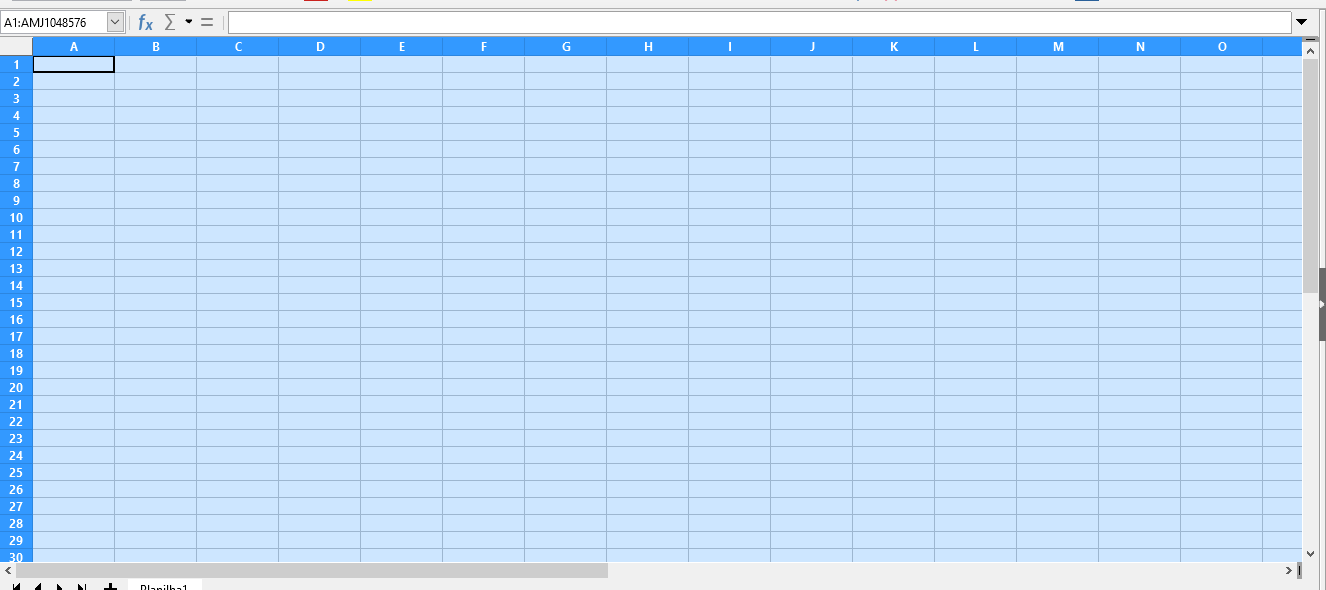
\includegraphics[width=1\linewidth]{Figuras/Ch06/fig16}
\end{frame}


\begin{frame}{Movimentação e seleção}
	\begin{block}{}
		\begin{itemize}
			\item Para \textbf{movimentar grupos de células}, pode-se \textbf{selecionar} o grupo de células, \textbf{clicar na borda} da seleção e \textbf{arrastar} até o destino.
		\end{itemize}
	\end{block}
	
	\bigskip
	
	\begin{minipage}{0.49\linewidth}
		\centering
		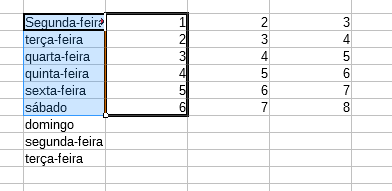
\includegraphics[width=1\linewidth]{Figuras/Ch06/fig17}
	\end{minipage}\hfill
	\begin{minipage}{0.49\linewidth}
		\centering
		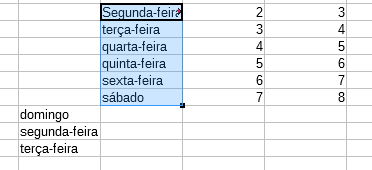
\includegraphics[width=1\linewidth]{Figuras/Ch06/fig18}
	\end{minipage}
\end{frame}


\begin{frame}{Ajuste de tamanho}
	\begin{block}{Células}
		\begin{itemize}
			\item Caso o \textbf{texto} de uma célula seja \textbf{maior} do que a \textbf{largura da coluna} em que se encontra, o texto ocupará o espaço da \textbf{próxima célula}, se ela estiver vazia.
			\item Esta ocupação \textbf{não significa} que o espaço da próxima célula foi \textbf{utilizado}.
		\end{itemize}
	\end{block}
	
	\centering
	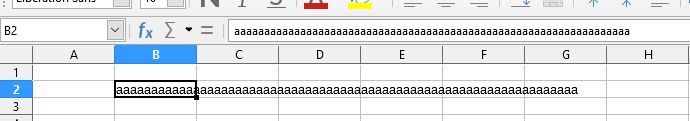
\includegraphics[width=0.7\linewidth]{Figuras/Ch06/fig19}
	
	\bigskip
	
	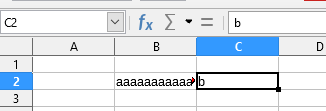
\includegraphics[width=0.5\linewidth]{Figuras/Ch06/fig20}
\end{frame}


\begin{frame}{Ajuste de tamanho}
	\begin{block}{Fileiras}
		\begin{itemize}
			\item Para \textbf{ajustar a largura} de uma única fileira, deve-se apontar o cursor no \textbf{limite} dela, \textbf{clicar}, \textbf{segurar} e \textbf{arrastar} (ou \textbf{clique duplo}).
		\end{itemize}
	\end{block}
	
	\centering
	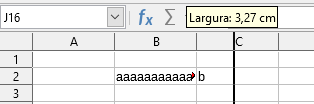
\includegraphics[width=0.5\linewidth]{Figuras/Ch06/fig21}
	
	\bigskip
	
	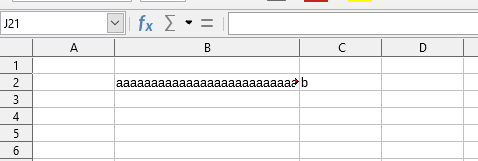
\includegraphics[width=0.7\linewidth]{Figuras/Ch06/fig22}
\end{frame}


\begin{frame}{Ajuste de tamanho}
	\begin{block}{Fileiras}
		\begin{itemize}
			\item Pode-se usar o recurso para \textbf{várias fileiras ao mesmo tempo}.
		\end{itemize}
	\end{block}
	
	\bigskip
	
	\centering
	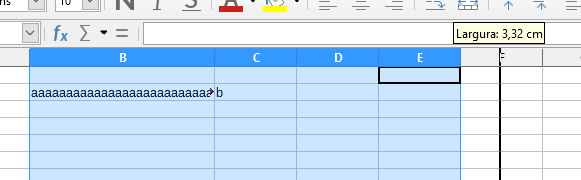
\includegraphics[width=0.6\linewidth]{Figuras/Ch06/fig23}
	
	\bigskip
	
	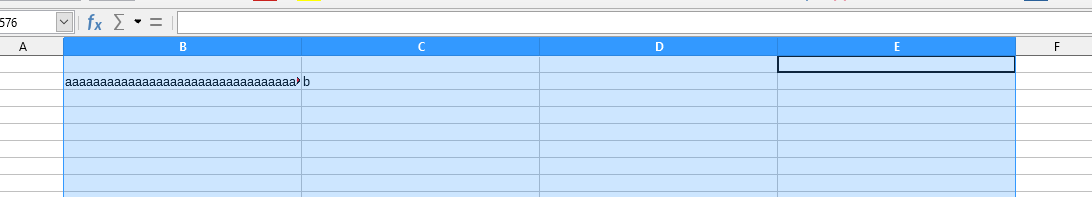
\includegraphics[width=0.7\linewidth]{Figuras/Ch06/fig24}
\end{frame}


\begin{frame}{Quebra de texto}
	\begin{block}{}
		\begin{itemize}
			\item Use esse recurso para textos \textbf{maiores} que a \textbf{largura da coluna}.
			\item Em vez de alterar a largura da coluna, a \textbf{altura da linha} que \textbf{será modificada}.
		\end{itemize}
	\end{block}
	
	\centering
	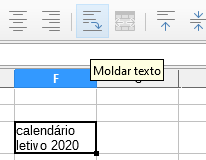
\includegraphics[width=0.5\linewidth]{Figuras/Ch06/fig25}
\end{frame}


\begin{frame}{Formatar célula}
	\begin{block}{}
		Transforma um grupo de células em uma célula única.
		\begin{enumerate}
			\item Selecione as células a serem mescladas;
			\item Formatar > Mesclar células > selecione a opção desejada
		\end{enumerate}
	\end{block}
	
	\medskip
	
	\begin{minipage}{0.49\linewidth}
		\centering
		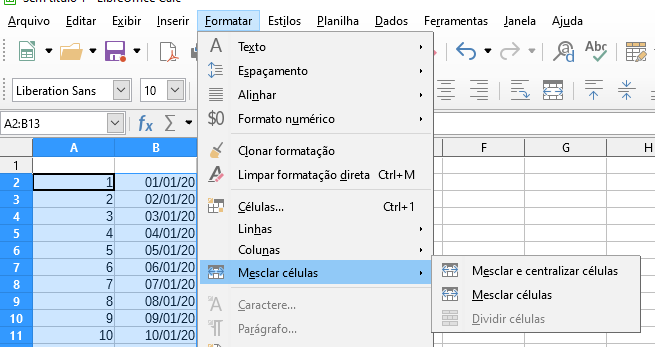
\includegraphics[width=1\linewidth]{Figuras/Ch06/fig28}
	\end{minipage}\hfill
	\begin{minipage}{0.49\linewidth}
		\centering
		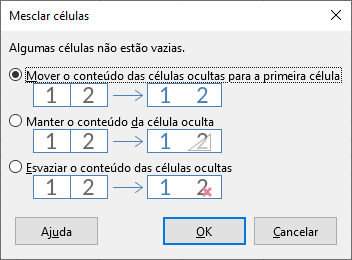
\includegraphics[width=1\linewidth]{Figuras/Ch06/fig29}
	\end{minipage}
\end{frame}


\begin{frame}{Formatar célula}
	\begin{minipage}{0.49\linewidth}
		\centering
		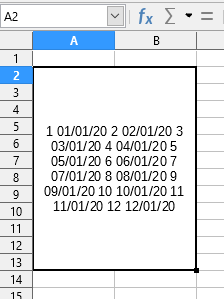
\includegraphics[width=0.9\linewidth]{Figuras/Ch06/fig30}
	\end{minipage}\hfill
	\begin{minipage}{0.49\linewidth}
		\centering
		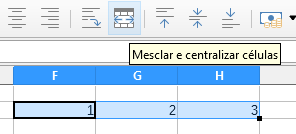
\includegraphics[width=1\linewidth]{Figuras/Ch06/fig31}
	\end{minipage}
\end{frame}


\begin{frame}{Formatar célula}
	\begin{block}{Tipo de formato numérico}
		Para a formatação da aparência das células de uma planilha, selecione as células desejadas.
		\begin{itemize}
			\item Formatar > Células...
			\item Selecione alguma das opções na barra de formatação.
		\end{itemize}
	\end{block}
	
	\begin{minipage}{0.49\linewidth}
		\centering
		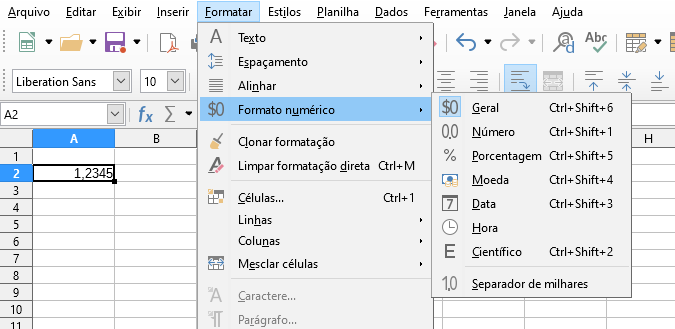
\includegraphics[width=1\linewidth]{Figuras/Ch06/fig32}
	\end{minipage}\hfill
	\begin{minipage}{0.49\linewidth}
		\centering
		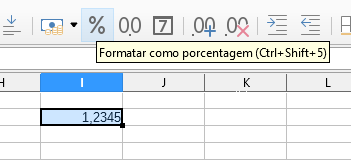
\includegraphics[width=1\linewidth]{Figuras/Ch06/fig33}
	\end{minipage}
\end{frame}


\begin{frame}{Formatar célula}
	\begin{block}{Tipo de borda}
		\begin{itemize}
			\item Muda as bordas em volta da célula.
		\end{itemize}
	\end{block}
	
	\begin{minipage}{0.49\linewidth}
		\centering
		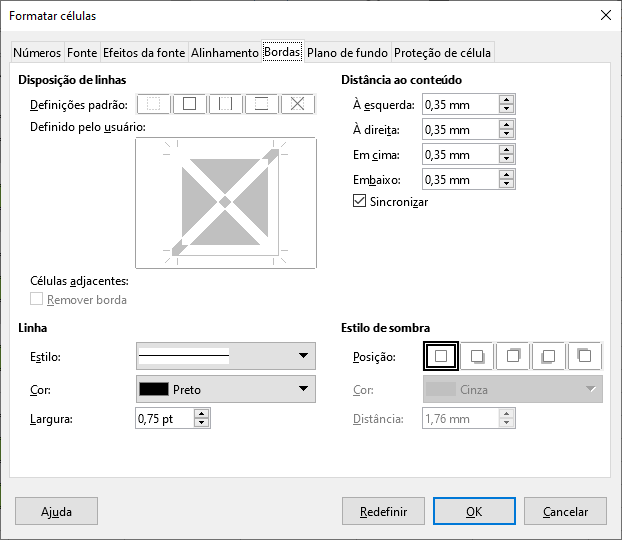
\includegraphics[width=1\linewidth]{Figuras/Ch06/fig34}
	\end{minipage}\hfill
	\begin{minipage}{0.49\linewidth}
		\centering
		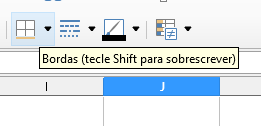
\includegraphics[width=1\linewidth]{Figuras/Ch06/fig35}
	\end{minipage}
\end{frame}


\begin{frame}{Formatar célula}
	\begin{block}{Formatação condicional}
		\begin{itemize}
			\item Permite \textbf{mudar a aparência} da célula baseando-se em \textbf{seu valor}.
		\end{itemize}
	\end{block}

	\centering
	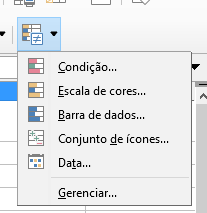
\includegraphics[width=0.5\linewidth]{Figuras/Ch06/fig36}
\end{frame}


\begin{frame}{Fórmulas}
	\begin{block}{}
		\begin{itemize}
			\item É possível utilizar diversas \textbf{funções}, e fazer \textbf{fórmulas matemáticas} úteis.
			\item Para fazer fórmulas devemos começar com um $ = $ ou clicar no botão Fórmula.
		\end{itemize}
	\end{block}

	\bigskip
	
	\begin{minipage}{0.3\linewidth}
		\centering
		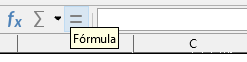
\includegraphics[width=1\linewidth]{Figuras/Ch06/fig38}
	\end{minipage}\hfill
	\begin{minipage}{0.3\linewidth}
		\centering
		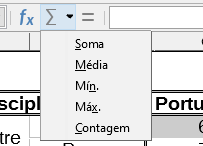
\includegraphics[width=1\linewidth]{Figuras/Ch06/fig39}
	\end{minipage}\hfill
	\begin{minipage}{0.3\linewidth}
		\centering
		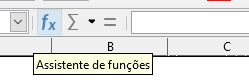
\includegraphics[width=1\linewidth]{Figuras/Ch06/fig40}
	\end{minipage}
\end{frame}


\begin{frame}{Fórmulas}
	\begin{block}{}
		\begin{itemize}
			\item Utilizando a função SOMA, por exemplo.
			\item A notação J2:J5 simplesmente diz que a função deve considerar todas as células, de J2 a J5.
		\end{itemize}
	\end{block}
	
	\begin{minipage}{0.45\linewidth}
		\centering
		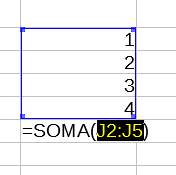
\includegraphics[width=1\linewidth]{Figuras/Ch06/fig42}
	\end{minipage}\hfill
	\begin{minipage}{0.45\linewidth}
		\centering
		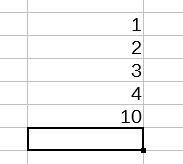
\includegraphics[width=1\linewidth]{Figuras/Ch06/fig43}
	\end{minipage}
\end{frame}


\begin{frame}{Fórmulas}
	\begin{block}{}
		\begin{itemize}
			\item Podemos também utilizar \textbf{operações simples}, como a \textbf{soma}, a \textbf{subtração}, a \textbf{multiplicação} e a \textbf{divisão}.
			\item E também podemos usar \textbf{valores decimais}.
		\end{itemize}
	\end{block}
	
	\centering
	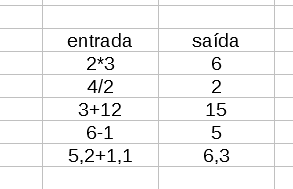
\includegraphics[width=0.6\linewidth]{Figuras/Ch06/fig44}
\end{frame}


\begin{frame}{Exemplo \#01 - Boletim}
	\begin{block}{}
		\begin{itemize}
			\item Só com essas ferramentas (fórmulas + célula condicional) podemos montar um \textbf{boletim simples}.
			\item Vamos começar inserindo uma disciplina qualquer, e uma estrutura onde vamos ter sua \textbf{média} em baixo.
		\end{itemize}
	\end{block}
	
	\bigskip
	
	\centering
	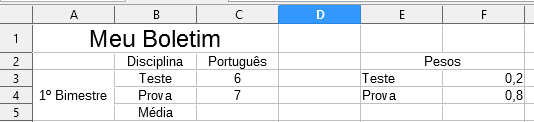
\includegraphics[width=1\linewidth]{Figuras/Ch06/fig44.1}
\end{frame}


\begin{frame}{Exemplo \#01 - Boletim}
	\begin{block}{}
		\begin{itemize}
			\item O grande poder das planilhas é que podemos fazer essas contas \textbf{automaticamente} com os valores inseridos.
			\item Para isso podemos digitar $ = $ e inserir a fórmula:
			
			\centerline{=C3*F4+C4*F5}
			\item Podemos inserir \textbf{endereços de células clicando sobre elas}.
		\end{itemize}
	\end{block}
	
	\bigskip
	
	\centering
	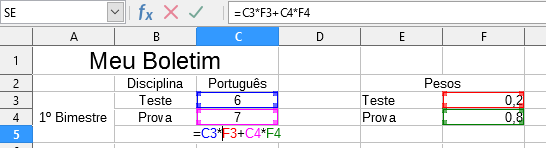
\includegraphics[width=1\linewidth]{Figuras/Ch06/fig44.2}
\end{frame}


\begin{frame}{Exemplo \#01 - Boletim}
	\begin{block}{}
		\begin{itemize}
			\item Para inserir outra disciplina, basta \textbf{inserir as notas} e puxar a aba de \textbf{autopreenchimento}.
		\end{itemize}
	\end{block}
	
	\centering
	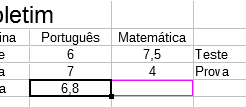
\includegraphics[width=0.8\linewidth]{Figuras/Ch06/fig44.3}
\end{frame}


\begin{frame}{Exemplo \#01 - Boletim}
	\begin{block}{}
		\begin{itemize}
			\item Repare que a fórmula ficou \textbf{errada}.
			\item Isso ocorre porque o Calc está tratando as células de pesos como se fossem \textbf{células normais} da nossa fórmula, porém elas são \textbf{constantes}.
		\end{itemize}
	\end{block}
	
	\centering
	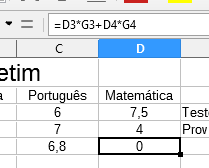
\includegraphics[width=0.6\linewidth]{Figuras/Ch06/fig44.4}
\end{frame}


\begin{frame}{Exemplo \#01 - Boletim}
	\begin{block}{}
		\begin{itemize}
			\item Para consertar isso, voltamos à fórmula inicial e inserimos um \$ no endereço dos pesos.
			\item Dessa forma, ao preencher as outras disciplinas com essa fórmula, o Calc sabe que \textbf{não deve alterar o endereço} dos pesos.
		\end{itemize}
	\end{block}
	
	\bigskip
	
	\centering
	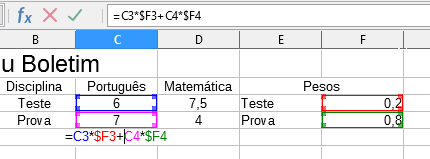
\includegraphics[width=1\linewidth]{Figuras/Ch06/fig44.5}
\end{frame}


\begin{frame}{Exemplo \#01 - Boletim}
	\begin{block}{}
		\begin{itemize}
			\item Agora podemos utilizar a \textbf{formatação condicional} para nos informar se nossa nota está \textbf{acima} ou \textbf{abaixo da média}.
		\end{itemize}
	\end{block}
	
	\bigskip
	
	\centering
	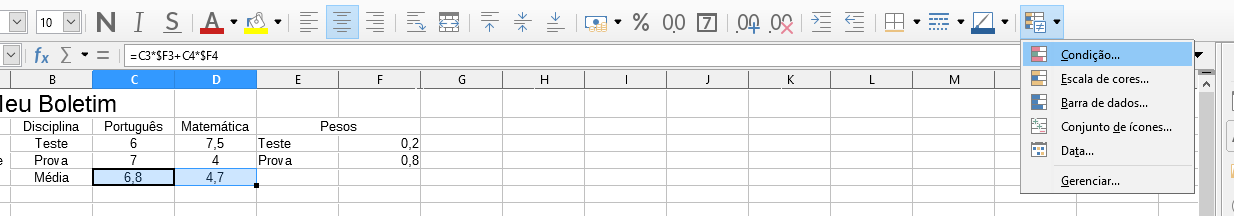
\includegraphics[width=1\linewidth]{Figuras/Ch06/fig44.6}
\end{frame}


\begin{frame}{Exemplo \#01 - Boletim}
	\begin{block}{}
		\begin{itemize}
			\item Primeiro devemos selecionar a condição desejada.
			\item No caso, se a nota for \textbf{menor que 6}, queremos que fique \textbf{vermelha}, portanto a \textbf{condição} é ser \textbf{menor que 6}.
		\end{itemize}
	\end{block}
	
	\bigskip
	
	\centering
	\includegraphics[width=0.8\linewidth]{Figuras/Ch06/fig44.7}
\end{frame}


\begin{frame}{Exemplo \#01 - Boletim}
	\begin{block}{}
		\begin{itemize}
			\item Agora, devemos escolher algum estilo para esse caso.
		\end{itemize}
	\end{block}
	
	\centering
	\includegraphics[width=0.6\linewidth]{Figuras/Ch06/fig44.8}
\end{frame}


\begin{frame}{Exemplo \#01 - Boletim}
	\begin{block}{}
		\begin{itemize}
			\item Agora adicionamos \textbf{outra formatação} para o caso da nota \textbf{igual ou acima da média}.
		\end{itemize}
	\end{block}
	
	\bigskip
	
	\centering
	\includegraphics[width=0.8\linewidth]{Figuras/Ch06/fig44.9}
\end{frame}


\begin{frame}{Exemplo \#01 - Boletim}
	\begin{block}{}
		\begin{itemize}
			\item Após configurar, basta clicar no OK.
		\end{itemize}
	\end{block}
	
	\centering
	\includegraphics[width=0.5\linewidth]{Figuras/Ch06/fig44.10}
\end{frame}


\begin{frame}{Exemplo \#01 - Boletim}
	\begin{block}{}
		\begin{itemize}
			\item Podemos identificar, agora, que a nota de \textbf{português} está \textbf{acima da média}, mas a nota de \textbf{matemática}, não.
		\end{itemize}
	\end{block}
	
	\bigskip
	
	\centering
	\includegraphics[width=1\linewidth]{Figuras/Ch06/fig44.11}
\end{frame}


\begin{frame}{Função SE}
	\begin{block}{Introdução}
		\begin{itemize}
			\item Outra forma de inserir \textbf{condições} em nossa tabela é usando a função \textbf{SE}.
			\item A diferença é que, para usá-la, devemos testar \textbf{condições matemáticas com código}.
			\item Pode parecer complexo, mas não é, e seguem algumas delas:
		\end{itemize}
	\end{block}
	
	\centering
	\includegraphics[width=0.6\linewidth]{Figuras/Ch06/fig44.12}
\end{frame}


\begin{frame}{Função SE}
	\begin{block}{Comparador $ = $}
		\begin{itemize}
			\item O comparador $ = $ vai retornar ``\textbf{verdadeiro}'' se, e somente se, as duas células comparadas forem \textbf{iguais}.
			\item Por exemplo, como $1\neq2$, o comparador nos diz que $ 1=2 $ é \textbf{falso}.
		\end{itemize}
	\end{block}
	
	\centering
	\includegraphics[width=0.6\linewidth]{Figuras/Ch06/fig44.13}
\end{frame}


\begin{frame}{Função SE}
	\begin{block}{Comparador $ > $}
		\begin{itemize}
			\item O comparador $ > $ vai retornar ``verdadeiro'' se, e somente se, o primeiro valor for \textbf{maior que} o segundo.
			\item Por exemplo, como $4=4$, o comparador nos diz que $ 4>4 $ é falso.
			\item O comparador $ < $ funciona de \textbf{forma análoga}.
		\end{itemize}
	\end{block}
	
	\centering
	\includegraphics[width=0.5\linewidth]{Figuras/Ch06/fig44.14}
\end{frame}


\begin{frame}{Função SE}
	\begin{block}{Comparador $ >= $}
		\begin{itemize}
			\item O comparador $ >= $ vai retornar ``verdadeiro'' se o primeiro valor for \textbf{maior \textit{ou} igual} ao segundo.
			\item Por exemplo, como $4=4$, o comparador nos diz que $ 4>=4 $ é verdadeiro.
			\item O comparador $ <= $ funciona de \textbf{forma análoga}.
		\end{itemize}
	\end{block}
	
	\centering
	\includegraphics[width=0.5\linewidth]{Figuras/Ch06/fig44.15}
\end{frame}


\begin{frame}{Função SE}
	\begin{block}{Comparador $ <> $}
		\begin{itemize}
			\item O comparador $ <> $ vai retornar ``verdadeiro'' se, e somente se, os valores forem \textbf{diferentes}.
			\item Por exemplo, como $5\neq6$, o comparador nos diz que $ 5<>6 $ é verdadeiro.
		\end{itemize}
	\end{block}
	
	\centering
	\includegraphics[width=0.6\linewidth]{Figuras/Ch06/fig44.16}
\end{frame}


\begin{frame}{Função SE}
	\begin{block}{}
		\begin{itemize}
			\item Vamos utilizar o \textbf{assistente de funções} para inserir a função SE.
		\end{itemize}
	\end{block}
	
	\bigskip
	
	\begin{minipage}{0.49\linewidth}
		\centering
		\includegraphics[width=1\linewidth]{Figuras/Ch06/fig41}
	\end{minipage}\hfill
	\begin{minipage}{0.49\linewidth}
		\centering
		\includegraphics[width=1\linewidth]{Figuras/Ch06/fig45}
	\end{minipage}
0\end{frame}


\begin{frame}{Função SE}
	\begin{block}{}
		\begin{itemize}
			\item A função SE precisa de uma \textbf{condição}, e depois devemos especificar o que fazer em \textbf{cada situação}:
			\begin{itemize}
				\item\normalsize caso a condição seja \textbf{verdadeira};
				\item\normalsize ou, caso seja \textbf{falsa}.
			\end{itemize}
		\end{itemize}
	\end{block}
	
	\centering
	\includegraphics[width=0.65\linewidth]{Figuras/Ch06/fig46}
\end{frame}


\begin{frame}{Função SE}
	\begin{block}{}
		\begin{itemize}
			\item No exemplo, estamos comparando se a célula de \textbf{cima} é \textbf{maior do que} a de \textbf{baixo}.
		\end{itemize}
	\end{block}

	\begin{minipage}{0.45\linewidth}
		\centering
		\includegraphics[width=1\linewidth]{Figuras/Ch06/fig47}
	\end{minipage}\hfill
	\begin{minipage}{0.45\linewidth}
		\centering
		\includegraphics[width=1\linewidth]{Figuras/Ch06/fig48}
	\end{minipage}
\end{frame}


\begin{frame}{Funções estatísticas}
	\begin{block}{Função MAIOR}
		\begin{itemize}
			\item Outras funções úteis são as \textbf{funções estatísticas}, que vão avaliar um \textbf{intervalo de números} e nos \textbf{informar} sobre ele.
			\item A função \textbf{MAIOR}, por exemplo, \textbf{organiza} os valores de uma lista em \textbf{ordem decrescente} e nos informa sobre \textbf{alguma posição}.
			\item No exemplo abaixo, estamos vendo o \textbf{maior valor} da lista, que foi \num{9,9} e, em seguida, vemos o \textbf{segundo maior valor}.
		\end{itemize}
	\end{block}
	
	\begin{minipage}{0.45\linewidth}
		\centering
		\includegraphics[width=1\linewidth]{Figuras/Ch06/fig50}
	\end{minipage}\hfill
	\begin{minipage}{0.45\linewidth}
		\centering
		\includegraphics[width=0.9\linewidth]{Figuras/Ch06/fig51}
	\end{minipage}
\end{frame}


\begin{frame}{Funções estatísticas}
	\begin{block}{Função MENOR}
		\begin{itemize}
			\item A função \textbf{MENOR} faz a mesma coisa, porém \textbf{ao contrário}.
		\end{itemize}
	\end{block}
	
	\bigskip
	
	\begin{minipage}{0.45\linewidth}
		\centering
		\includegraphics[width=1\linewidth]{Figuras/Ch06/fig52}
	\end{minipage}\hfill
	\begin{minipage}{0.45\linewidth}
		\centering
		\includegraphics[width=1\linewidth]{Figuras/Ch06/fig53}
	\end{minipage}
\end{frame}


\begin{frame}{Funções estatísticas}
	\begin{block}{Funções MÁXIMO e MÍNIMO}
		\begin{itemize}
			\item Estas vão dar somente os \textbf{valores extremos} do intervalo.
		\end{itemize}
	\end{block}
	
	\bigskip
	
	\begin{minipage}{0.45\linewidth}
		\centering
		\includegraphics[width=1\linewidth]{Figuras/Ch06/fig54}
	\end{minipage}\hfill
	\begin{minipage}{0.45\linewidth}
		\centering
		\includegraphics[width=1\linewidth]{Figuras/Ch06/fig55}
	\end{minipage}
\end{frame}


\begin{frame}{Exemplo \#02 - Boletim finalizado}
	\begin{block}{}
		\begin{itemize}
			\item É possível fazer planilhas bastante úteis com os recursos apresentados.
		\end{itemize}
	\end{block}
	
	\medskip
	
	\centering
	\includegraphics[width=1\linewidth]{Figuras/Ch06/fig49}
\end{frame}


\section*{Exercícios}
\frame{
	\frametitle{Exercícios}
	\begin{block}{}
		01. Imagine a situação em que você gerencia uma loja. Quais utilidades o Calc teria para você?
		
		\medskip
		
		02. Você tem problemas com notas ou com dinheiro? Mesmo que não tenha, monte uma planilha para te ajudar a se organizar com essas coisas.
	\end{block}
}

\section*{Referências}

\frame{
	\frametitle{Referências e Exercícios Complementares}
	\begin{itemize}
		\item Introdução ao LibreOffice, \href{https://documentation.libreoffice.org/assets/Uploads/Documentation/pt-br/GS50/GS50-IntroducaoLO-5.0-ptbr.pdf}{Apostila de uso livre}.
	\end{itemize}
	%\centering{\alert{Página 36 - \textbf{1.6.1 até 1.6.5, 1.6.17 até 1.6.19}}} \\
	%	\centering{\alert{Lista de exercícios 01}}
}